\section{Label Transition System}

\emph{Reprotool} users work by editing use-cases using our use-case editor. The in-memory representation of actual use-cases are java
objects that are modelled according to our use-case model. (See a simplified view of the model in Figure~\ref{fig:ReprotoolUCModel})
While this model is very useful, it is also quite complex. In some cases we find it helpful to take just a simplified view of a
use-case and consider it a state machine. Every use-case has a main scenario that has a first use-case step, a last step (They could,
however, be the same step) and possibly some other steps. That is analogical to a state machine that has a initial state, an accepting
state and possibly some other states. The model that describes the building blocks of this state machine is based on the EMF and is
called \emph{Label Transition System}.

We use the \emph{LTS} in \emph{Reprotool} when we create NuSMV state machines from use-cases that are used during the NuSMV
verification. We also take advantage of the \emph{LTS} when we create a graphical view of a use-case in the outline view of the
use-case editor. The \emph{LTS} model is depicted in the following figure.

\begin{figure}[ht]
  \centering
  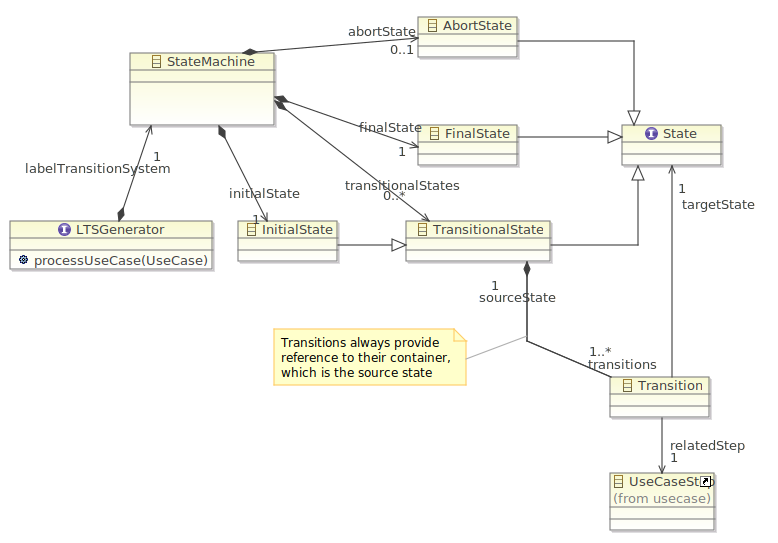
\includegraphics[width=450pt]{images/lts}
  \caption{\emph{LTS} model}
  \label{fig:ReprotoolLTSModel}
\end{figure}

Now, we will describe in more detail the way how the \emph{LTS} state machine is constructed from some use-case \emph{U}.

\subsection{Variation scenario}
If a use-case step \emph{s} has a variation scenario specified, that means either the step \emph{s} is taken, or its variation scenario is
taken. Not both of them. After the variation scenario is performed, the execution continues after the step \emph{s}. (But if the
last step of the variation scenario has a \emph{goto} action specified, the execution continues at step that is specified as
\emph{goto} target.)

This is depicted in the next figure that shows a simple use-case \emph{U} and the use-case \emph{U\'} with a variation
scenario added to the second step (the red one). The variation scenario is two steps long.
Notice the placement of the variation branch in the picture and also notice that an additional transition \emph{t} (the blue one)
has been added to the \emph{LTS} diagram that determines where the execution continues after the variation scenario. This transition
\emph{t} is not directly related to any of the use-case steps of the use-case \emph{U}. All other \emph{LTS} transitions have a
corresponding use-case step in the use-case \emph{U} or in the variation scenario.

\begin{figure}[ht]
  \centering
  
\includegraphics[width=200pt]{images/variation}
  \caption{Use-case \emph{U} and use-case \emph{U\'} with a variation scenario added}
  \label{fig:VariationScenario}
\end{figure}

\subsection{Extension scenario}
If a use-case step \emph{s} has an extension scenario specified, that means after the step \emph{s} is taken, the extension scenario
might be taken. After the extension scenario is performed, the execution continues after the step \emph{s}. (But if the
last step of the extension scenario has a \emph{goto} action specified, the execution continues at step that is specified as
\emph{goto} target.)

This is shown in the next figure that shows a simple use-case \emph{U} and the use-case \emph{U\'} with an extension scenario added
to the first step (the red one). The extension scenario is two steps long.
Notice the placement of the extension branch in the picture and also notice that two additional transitions (the blue ones) have been
added to the \emph{LTS} diagram. One blue transition has been added at the end of the extension scenario and it determines where
the execution continues after the extension scenario is performed. The second blue transition has been added between the red and the
violet use case step - these are consecutive in the original use-case \emph{U}. This second blue transition is taken if the extension
scenario is not taken. Again, the blue transitions do not have a corresponding use-case step. All other transition have one - either
in the original use-case \emph{U} or in the extension scenario.

\begin{figure}[ht]
  \centering
  
\includegraphics[width=200pt]{images/extension}
  \caption{Use-case \emph{U} and use-case \emph{U\'} with an extension scenario added}
  \label{fig:ExtensionScenario}
\end{figure}

\subsection{LTS visualisation}